% Options for packages loaded elsewhere
\PassOptionsToPackage{unicode}{hyperref}
\PassOptionsToPackage{hyphens}{url}
%
\documentclass[
  donotrepeattitle,doc, 12pt, a4paper,floatsintext]{apa7}

\usepackage{graphicx}
\makeatletter
\def\maxwidth{\ifdim\Gin@nat@width>\linewidth\linewidth\else\Gin@nat@width\fi}
\def\maxheight{\ifdim\Gin@nat@height>\textheight\textheight\else\Gin@nat@height\fi}
\makeatother
% Scale images if necessary, so that they will not overflow the page
% margins by default, and it is still possible to overwrite the defaults
% using explicit options in \includegraphics[width, height, ...]{}
\setkeys{Gin}{width=\maxwidth,height=\maxheight,keepaspectratio}
% Set default figure placement to htbp
\makeatletter
\def\fps@figure{htbp}
\makeatother
\setlength{\emergencystretch}{3em} % prevent overfull lines
\providecommand{\tightlist}{%
  \setlength{\itemsep}{0pt}\setlength{\parskip}{0pt}}
\setcounter{secnumdepth}{5}
% Make \paragraph and \subparagraph free-standing
\ifx\paragraph\undefined\else
  \let\oldparagraph\paragraph
  \renewcommand{\paragraph}[1]{\oldparagraph{#1}\mbox{}}
\fi
\ifx\subparagraph\undefined\else
  \let\oldsubparagraph\subparagraph
  \renewcommand{\subparagraph}[1]{\oldsubparagraph{#1}\mbox{}}
\fi
\ifLuaTeX
\usepackage[bidi=basic]{babel}
\else
\usepackage[bidi=default]{babel}
\fi
\babelprovide[main,import]{english}
% get rid of language-specific shorthands (see #6817):
\let\LanguageShortHands\languageshorthands
\def\languageshorthands#1{}
% Manuscript styling
\usepackage{upgreek}
\captionsetup{font=singlespacing,justification=justified}

% Table formatting
\usepackage{longtable}
\usepackage{lscape}
% \usepackage[counterclockwise]{rotating}   % Landscape page setup for large tables
\usepackage{multirow}		% Table styling
\usepackage{tabularx}		% Control Column width
\usepackage[flushleft]{threeparttable}	% Allows for three part tables with a specified notes section
\usepackage{threeparttablex}            % Lets threeparttable work with longtable

% Create new environments so endfloat can handle them
% \newenvironment{ltable}
%   {\begin{landscape}\centering\begin{threeparttable}}
%   {\end{threeparttable}\end{landscape}}
\newenvironment{lltable}{\begin{landscape}\centering\begin{ThreePartTable}}{\end{ThreePartTable}\end{landscape}}

% Enables adjusting longtable caption width to table width
% Solution found at http://golatex.de/longtable-mit-caption-so-breit-wie-die-tabelle-t15767.html
\makeatletter
\newcommand\LastLTentrywidth{1em}
\newlength\longtablewidth
\setlength{\longtablewidth}{1in}
\newcommand{\getlongtablewidth}{\begingroup \ifcsname LT@\roman{LT@tables}\endcsname \global\longtablewidth=0pt \renewcommand{\LT@entry}[2]{\global\advance\longtablewidth by ##2\relax\gdef\LastLTentrywidth{##2}}\@nameuse{LT@\roman{LT@tables}} \fi \endgroup}

% \setlength{\parindent}{0.5in}
% \setlength{\parskip}{0pt plus 0pt minus 0pt}

% Overwrite redefinition of paragraph and subparagraph by the default LaTeX template
% See https://github.com/crsh/papaja/issues/292
\makeatletter
\renewcommand{\paragraph}{\@startsection{paragraph}{4}{\parindent}%
  {0\baselineskip \@plus 0.2ex \@minus 0.2ex}%
  {-1em}%
  {\normalfont\normalsize\bfseries\itshape\typesectitle}}

\renewcommand{\subparagraph}[1]{\@startsection{subparagraph}{5}{1em}%
  {0\baselineskip \@plus 0.2ex \@minus 0.2ex}%
  {-\z@\relax}%
  {\normalfont\normalsize\itshape\hspace{\parindent}{#1}\textit{\addperi}}{\relax}}
\makeatother

% \usepackage{etoolbox}
\makeatletter
\patchcmd{\HyOrg@maketitle}
  {\section{\normalfont\normalsize\abstractname}}
  {\section*{\normalfont\normalsize\abstractname}}
  {}{\typeout{Failed to patch abstract.}}
\patchcmd{\HyOrg@maketitle}
  {\section{\protect\normalfont{\@title}}}
  {\section*{\protect\normalfont{\@title}}}
  {}{\typeout{Failed to patch title.}}
\makeatother

\usepackage{xpatch}
\makeatletter
\xapptocmd\appendix
  {\xapptocmd\section
    {\addcontentsline{toc}{section}{\appendixname\ifoneappendix\else~\theappendix\fi\\: #1}}
    {}{\InnerPatchFailed}%
  }
{}{\PatchFailed}
\keywords{keywords}
\usepackage{csquotes}
\geometry{a4paper, left = 4cm, right = 2.5cm, top = 2cm, bottom = 4cm}


\usepackage[titles]{tocloft}
\cftpagenumbersoff{figure}
\renewcommand{\cftfigpresnum}{\itshape\figurename\enspace}
\renewcommand{\cftfigaftersnum}{.\space}
\setlength{\cftfigindent}{0pt}
\setlength{\cftafterloftitleskip}{0pt}
\settowidth{\cftfignumwidth}{Figure 10.\qquad}
\cftpagenumbersoff{table}
\renewcommand{\cfttabpresnum}{\itshape\tablename\enspace}
\renewcommand{\cfttabaftersnum}{.\space}
\setlength{\cfttabindent}{0pt}
\setlength{\cftafterloftitleskip}{0pt}
\settowidth{\cfttabnumwidth}{Table 10.\qquad}
\setcounter{tocdepth}{3}
\linespread{1.2}
\usepackage{fancyhdr}
\interfootnotelinepenalty=10000
\usepackage{setspace}
\newcommand{\HRule}{\rule{\linewidth}{0.25mm}}
\raggedbottom
\captionsetup[figure]{textformat=empty}
\usepackage{pdflscape}
\usepackage{threeparttablex}
\ifLuaTeX
  \usepackage{selnolig}  % disable illegal ligatures
\fi
\IfFileExists{bookmark.sty}{\usepackage{bookmark}}{\usepackage{hyperref}}
\IfFileExists{xurl.sty}{\usepackage{xurl}}{} % add URL line breaks if available
\urlstyle{same} % disable monospaced font for URLs
\hypersetup{
  pdftitle={Power motivations and risk sensitivity and tolerance.},
  pdfauthor={Ithurburn, Andrew1, Pedersen M.E., Julie1, \& Moore, Adam1},
  pdflang={en-EN},
  pdfkeywords={keywords},
  hidelinks,
  pdfcreator={LaTeX via pandoc}}

\title{Power motivations and risk sensitivity and tolerance.}
\author{Ithurburn, Andrew\textsuperscript{1}, Pedersen M.E., Julie\textsuperscript{1}, \& Moore, Adam\textsuperscript{1}}
\date{}


\shorttitle{DoPL and DOSPERT}

\authornote{

The authors made the following contributions. Ithurburn, Andrew: ; Moore, Adam: Writing - Review \& Editing, Supervision.

Correspondence concerning this article should be addressed to Ithurburn, Andrew, 7 George Square, Edinburgh, EH8 9JZ. E-mail: \href{mailto:a.ithurburn@sms.ed.ac.uk}{\nolinkurl{a.ithurburn@sms.ed.ac.uk}}

}

\affiliation{\vspace{0.5cm}\textsuperscript{1} The University of Edinburgh}

\abstract{%
In the present research, we sought to examine through two experiments the interaction between power motives (dominance, prestige, and leadership) and risk taking behaviors. In study 1 we discovered that individuals high in dominance power motive were more likley to enage in financiall, ethical and health and safety based risk sitations.
}



\begin{document}
\maketitle

\begin{figure}
\centering
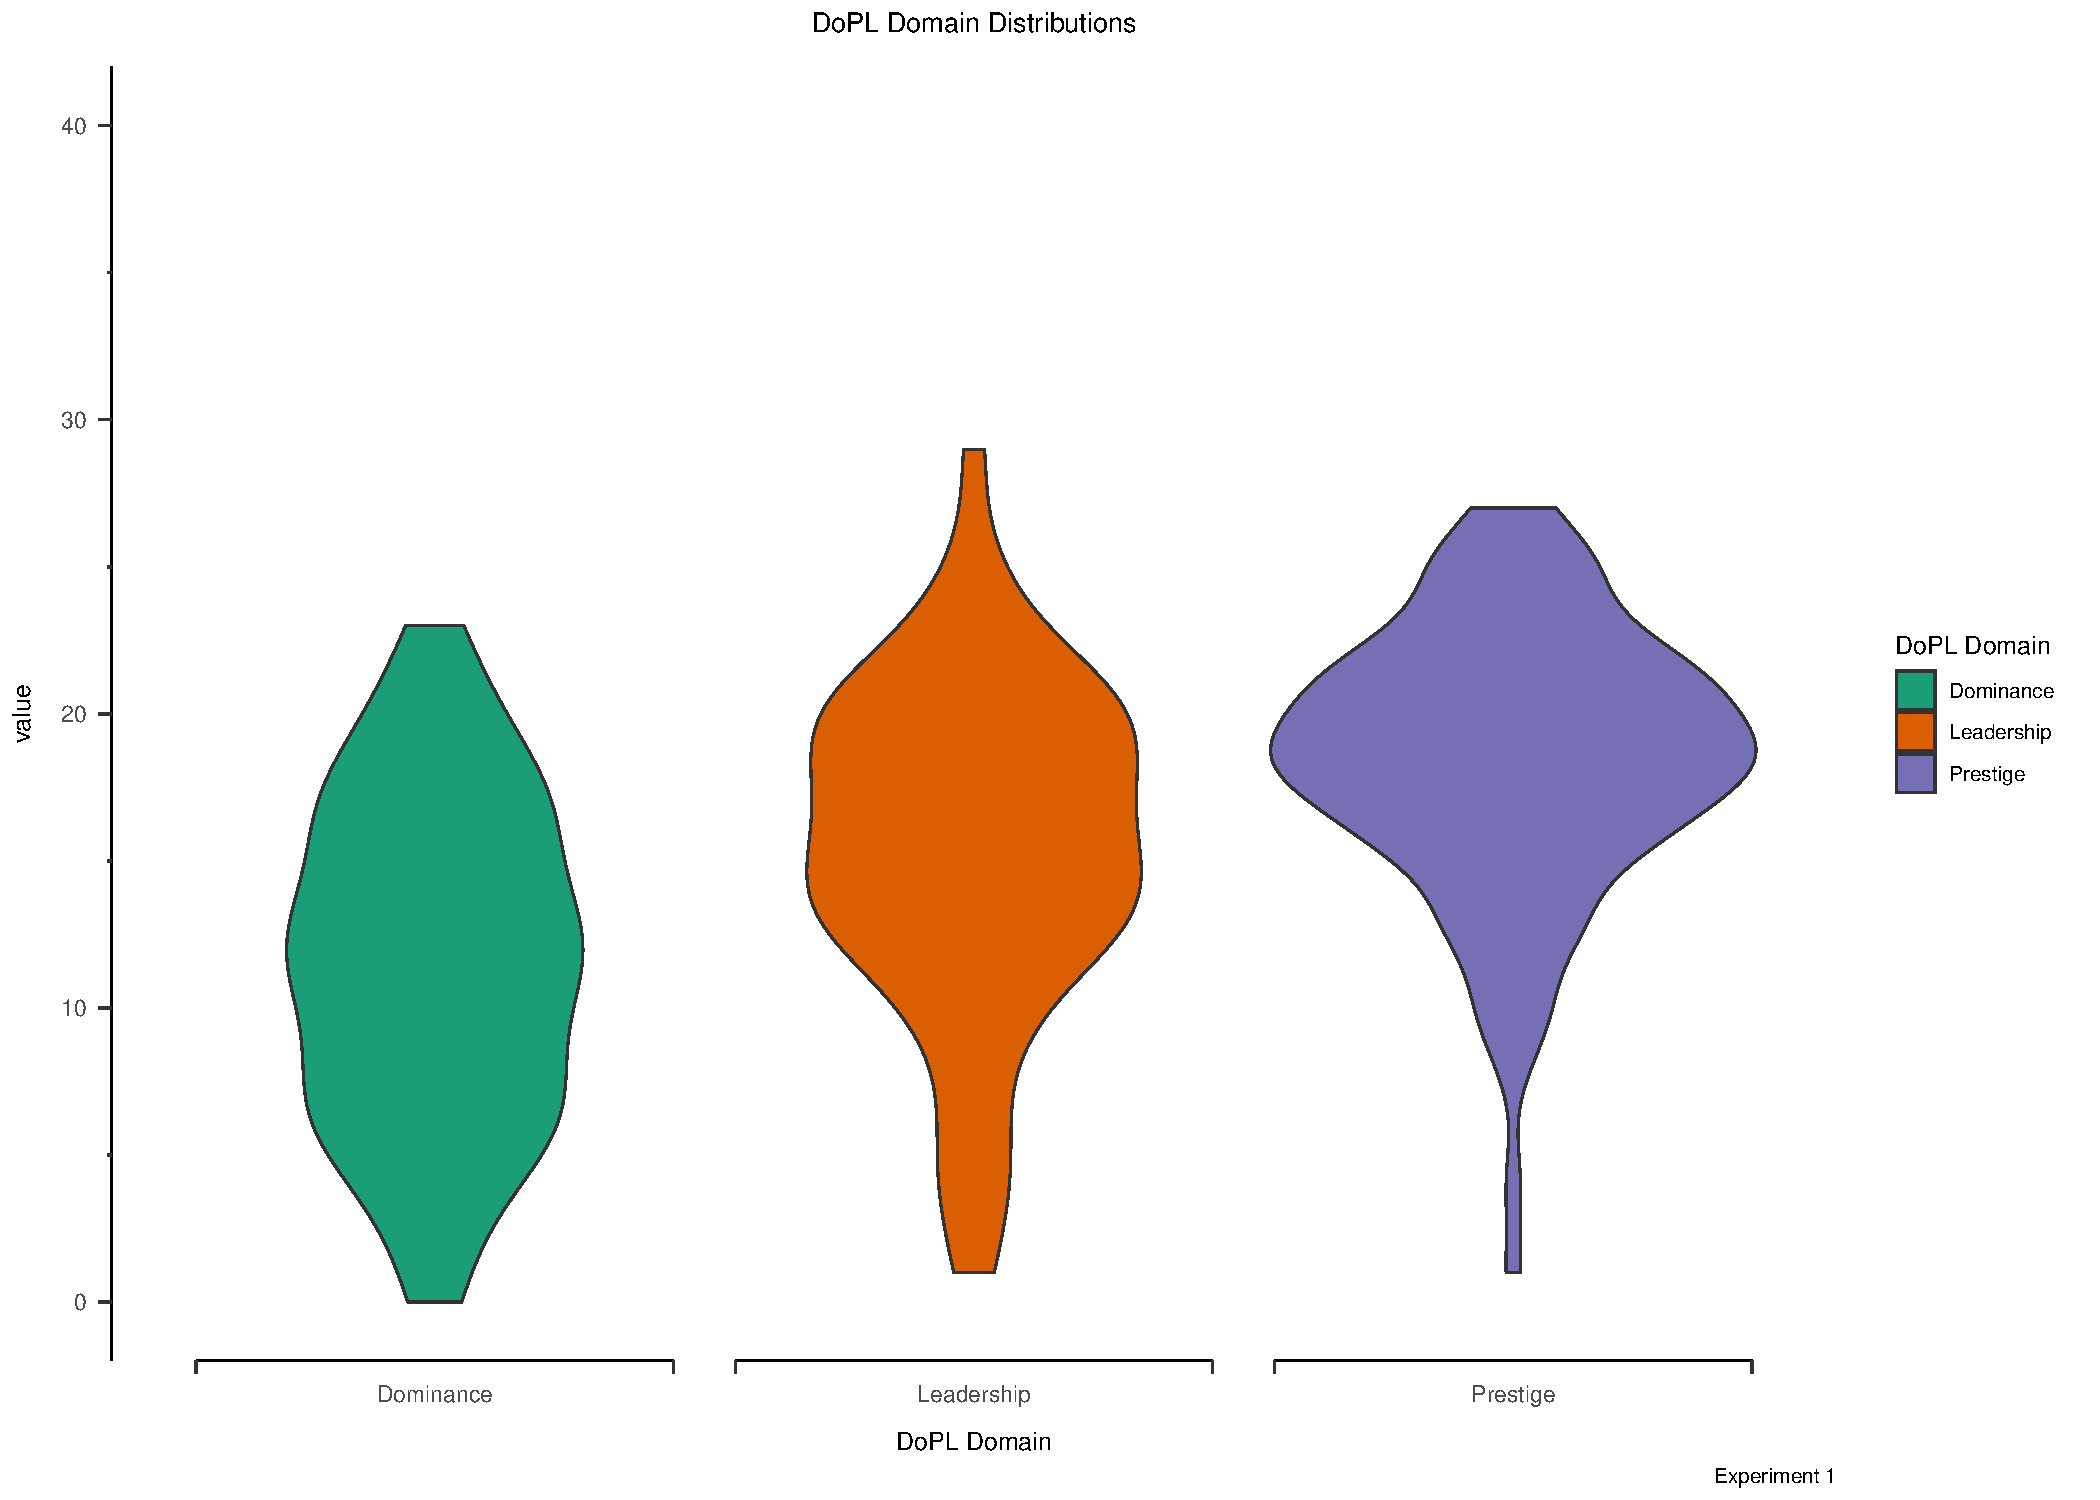
\includegraphics{/Output_Files/Chapter-2-graphs_files/figure-latex/DoPL-Experiment-1-1.pdf}
\caption{\label{fig:DoPL-Experiment-1}Violin plot visually showing the distribution of dominance, prestige, and leadership of participants in experiment 1. As seen in the figure, of participants within each power orientation dominance oriented people are more evenly distributed while those that were more prestige and leadership oriented were tended to be more prestigous oriented than others.}
\end{figure}

\begin{figure}

{\centering 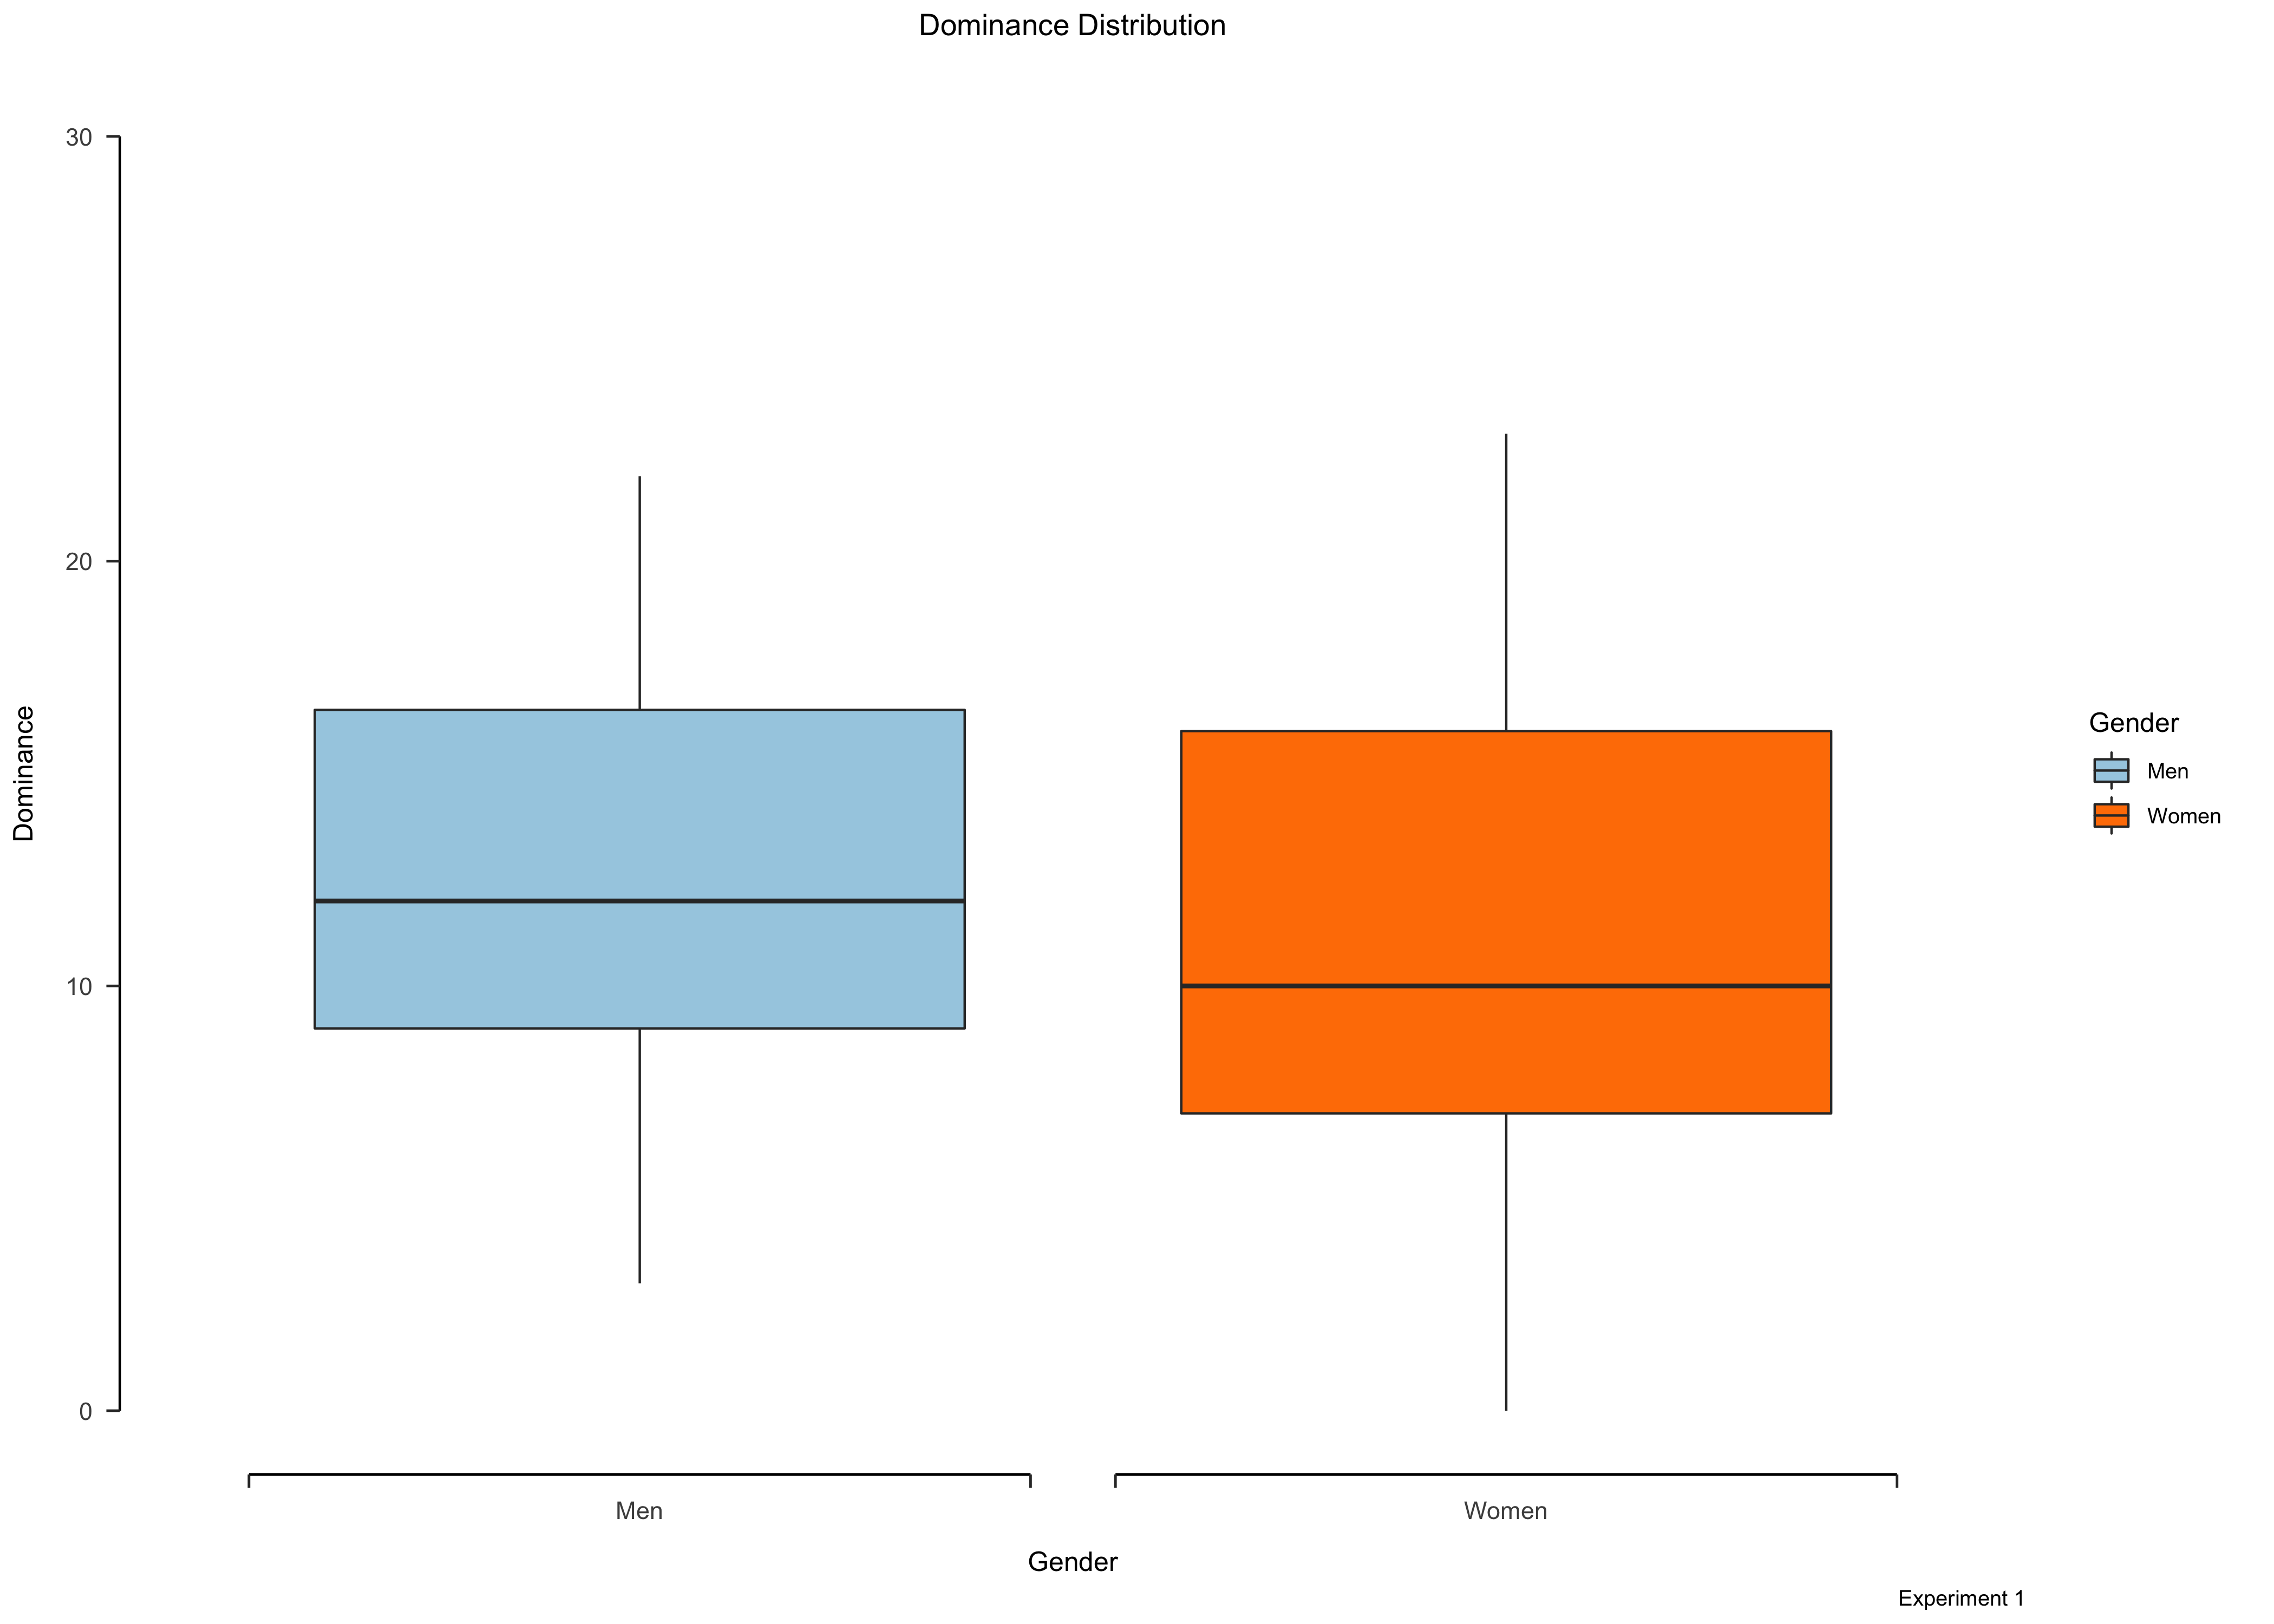
\includegraphics{/Output_Files/Chapter-2-graphs_files/figure-latex/DominanceExperiment1-1} 

}

\caption{Depicted is the gender distribution of Men and Women with regard to level of dominance. As can be seen, men are slightly higher in dominance then women.}\label{fig:DominanceExperiment1}
\end{figure}

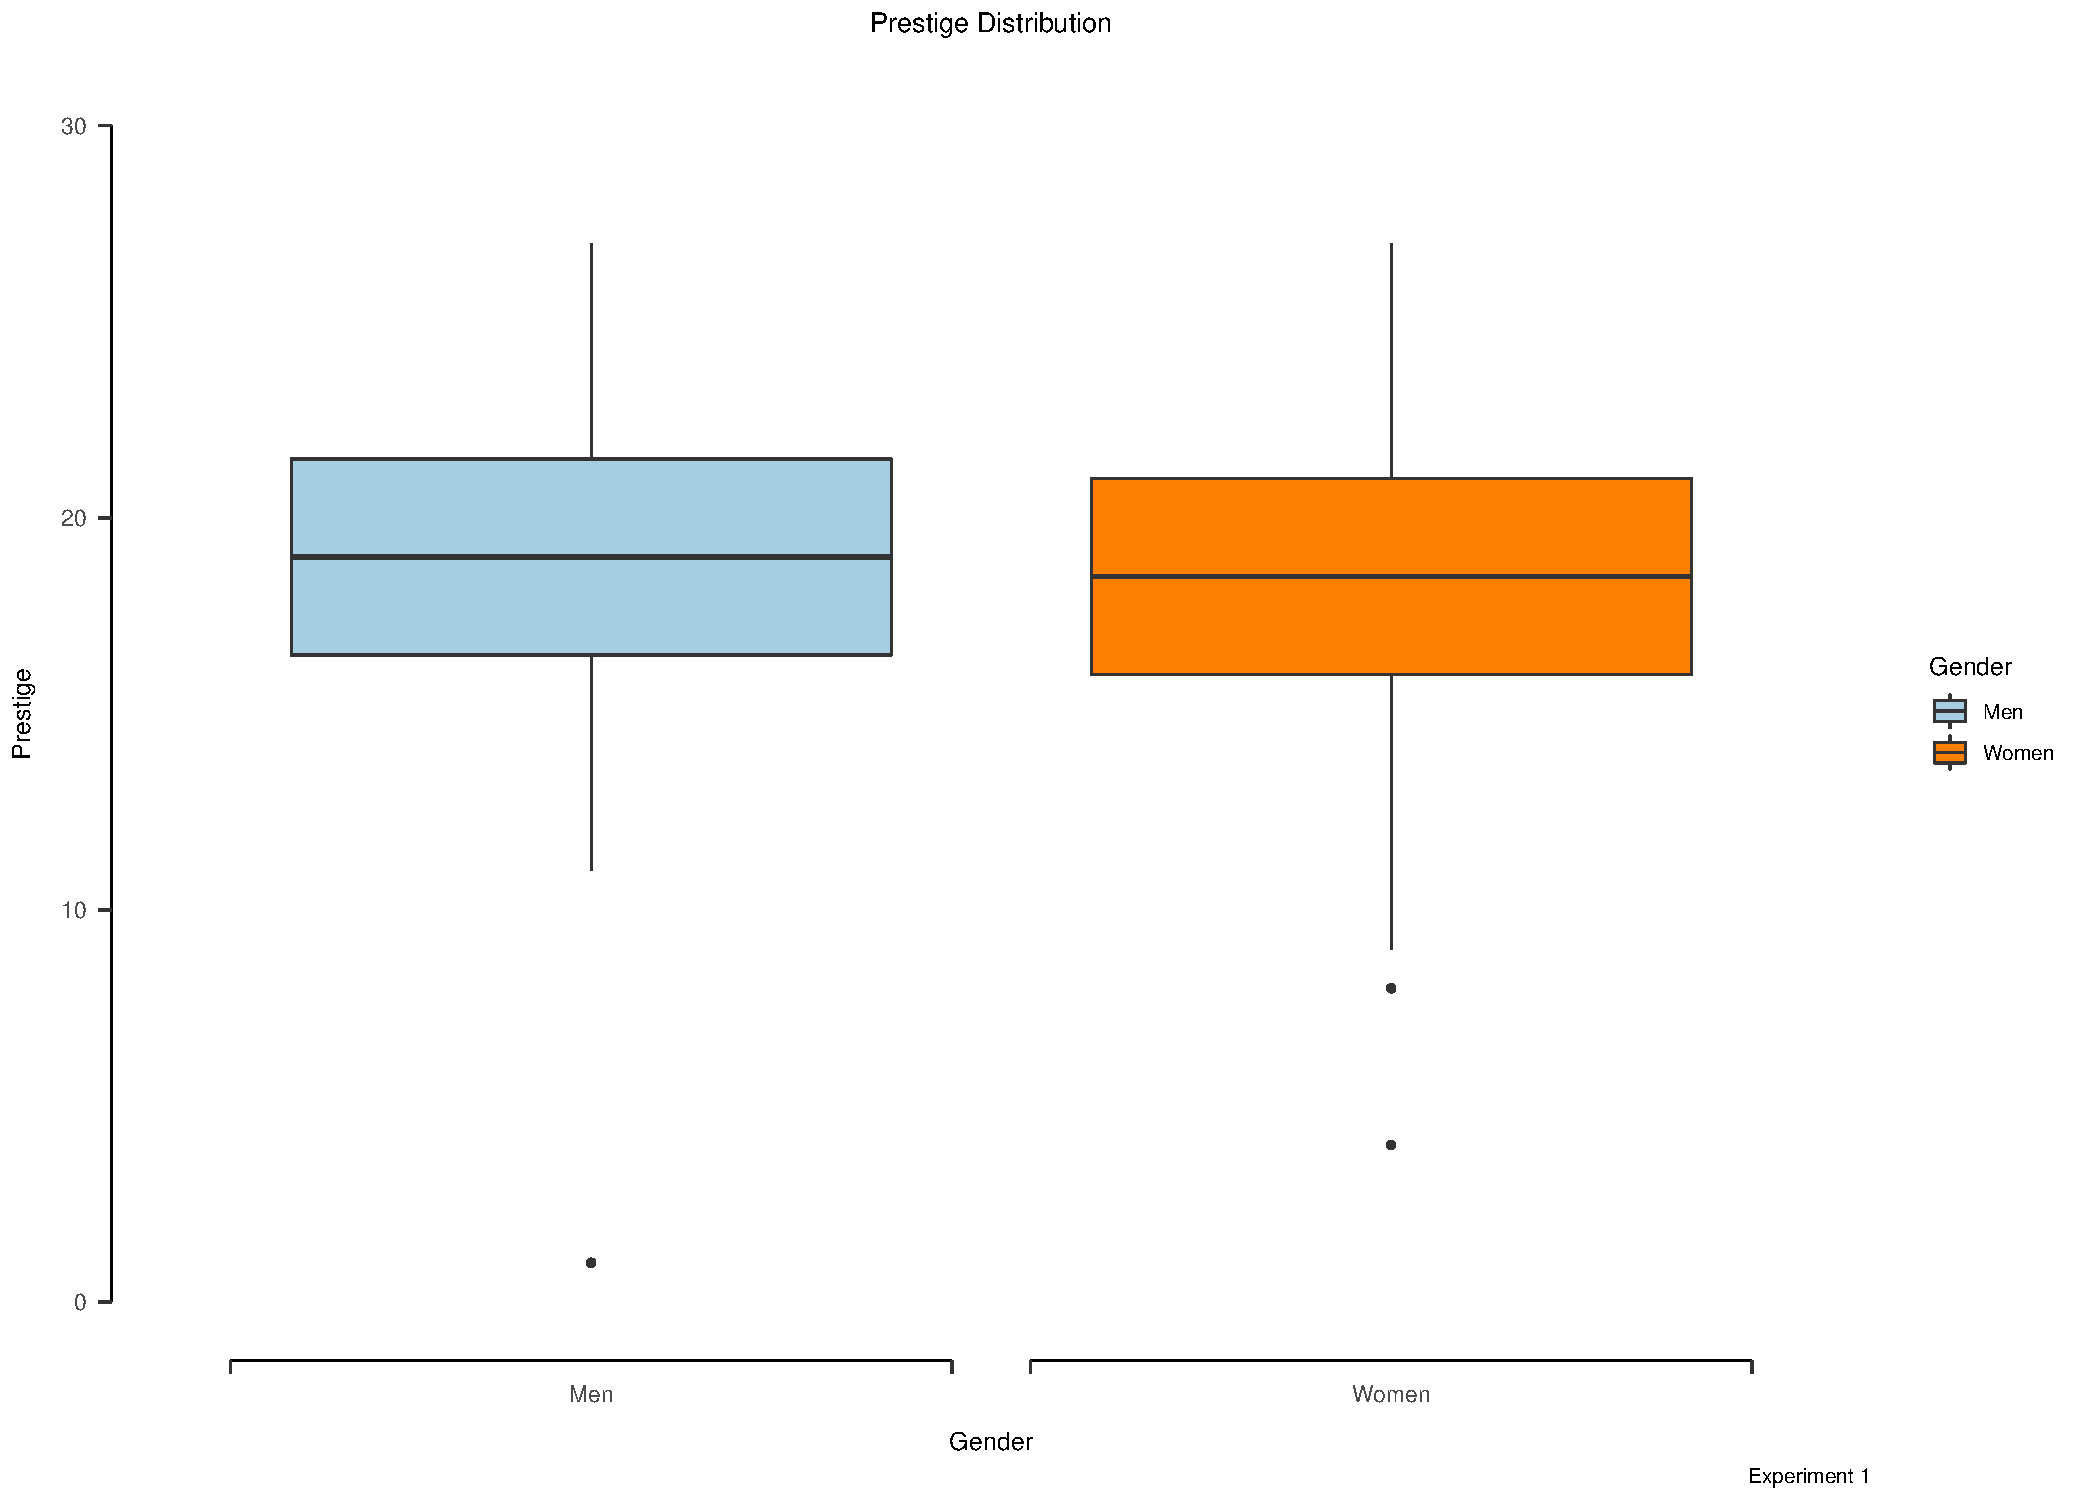
\includegraphics{/Output_Files/Chapter-2-graphs_files/figure-latex/PrestigeExperiment1-1.pdf}
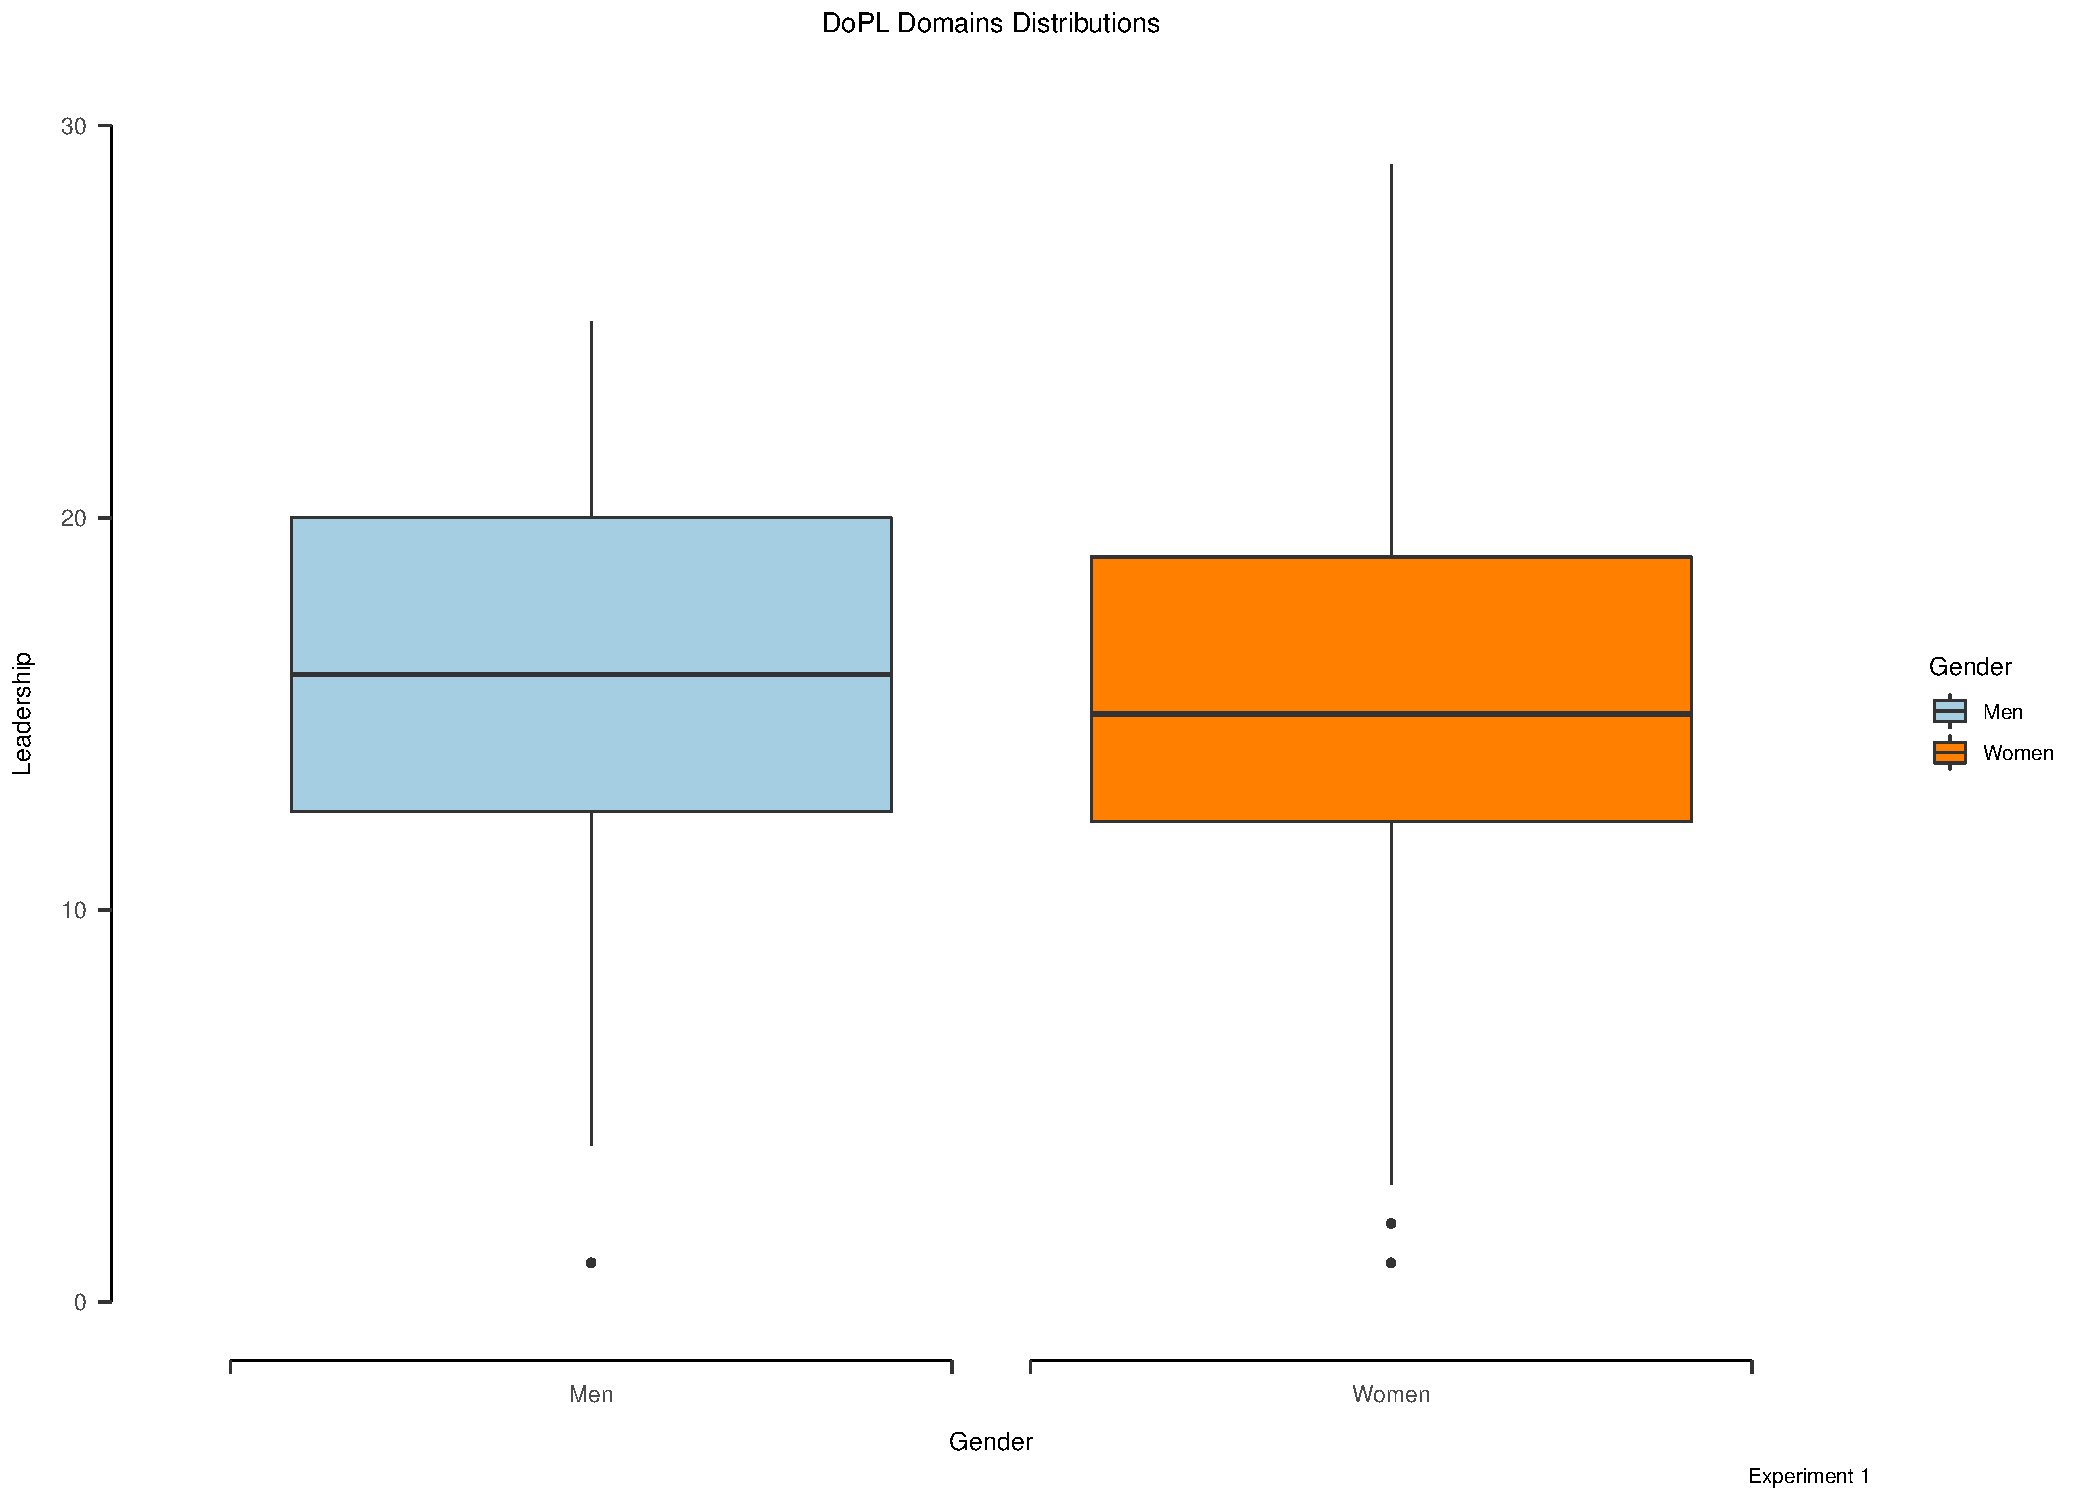
\includegraphics{/Output_Files/Chapter-2-graphs_files/figure-latex/LeadershipExperiment1-1.pdf}
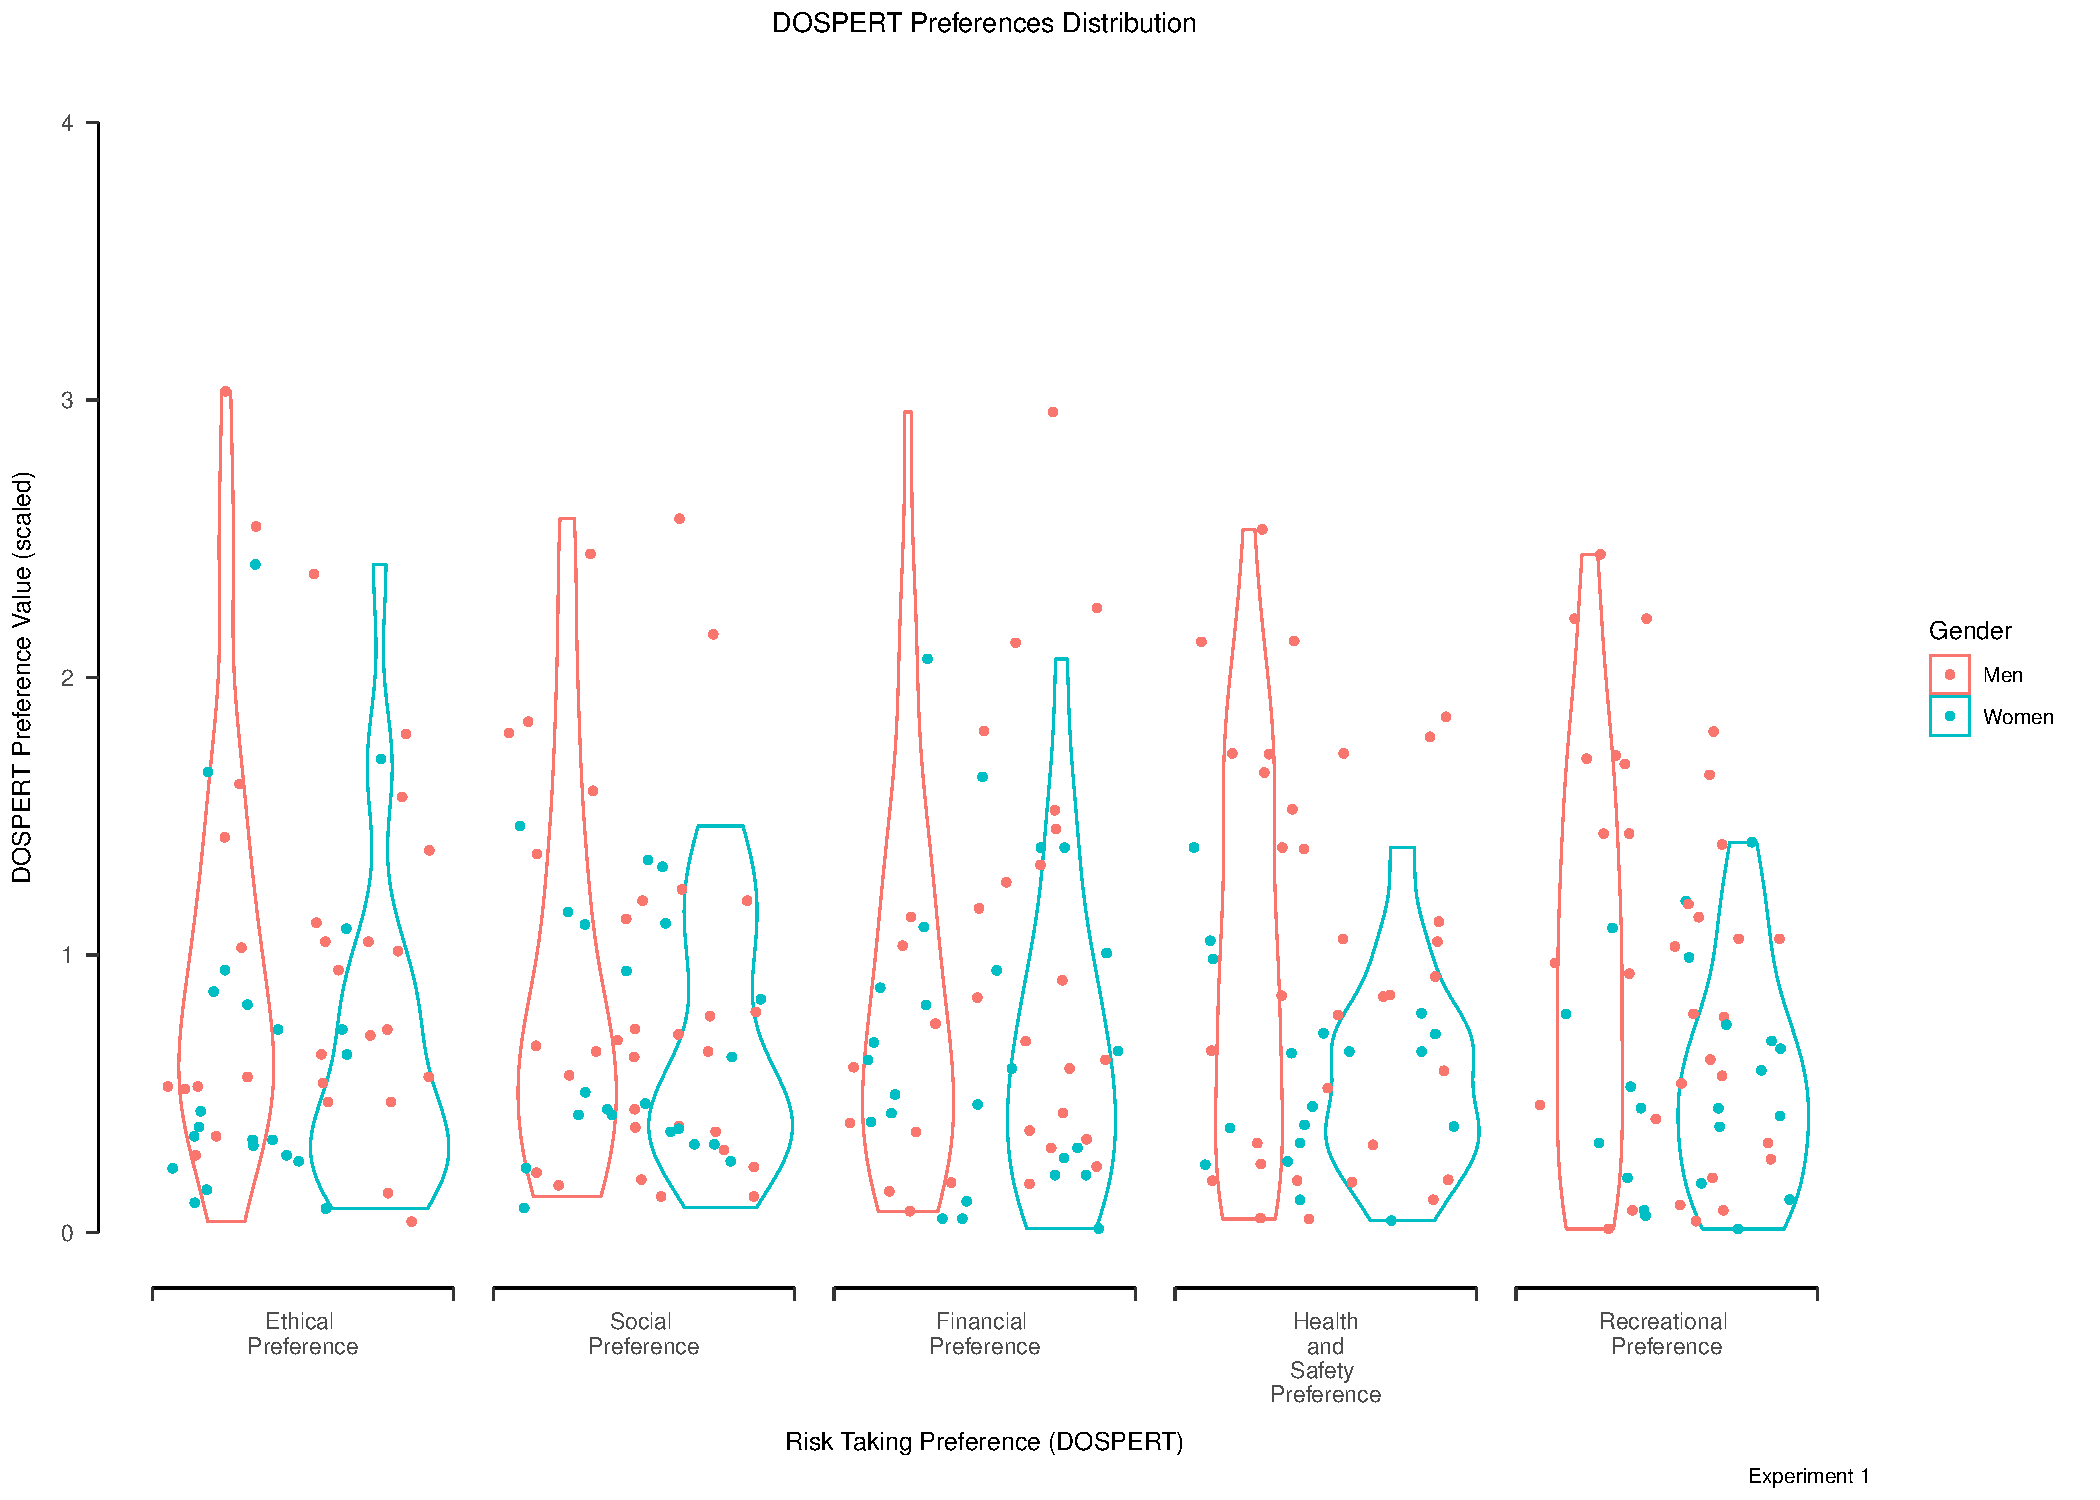
\includegraphics{/Output_Files/Chapter-2-graphs_files/figure-latex/DOSPERT-Preferences-GenderExperiment1-1.pdf}
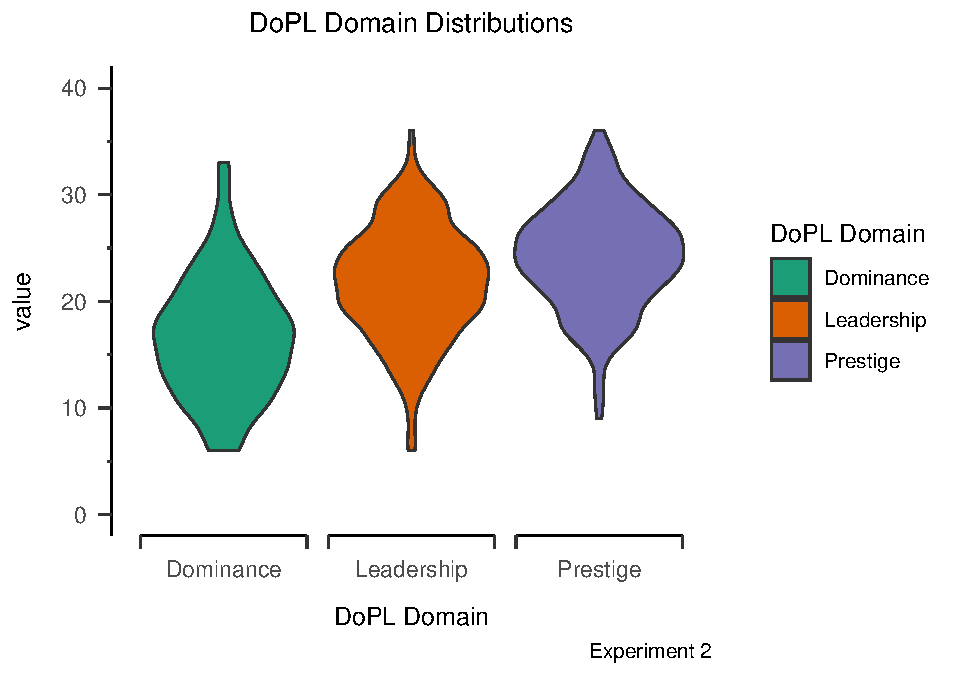
\includegraphics{/Output_Files/Chapter-2-graphs_files/figure-latex/DoPLDomainsExperiment2-1.pdf}
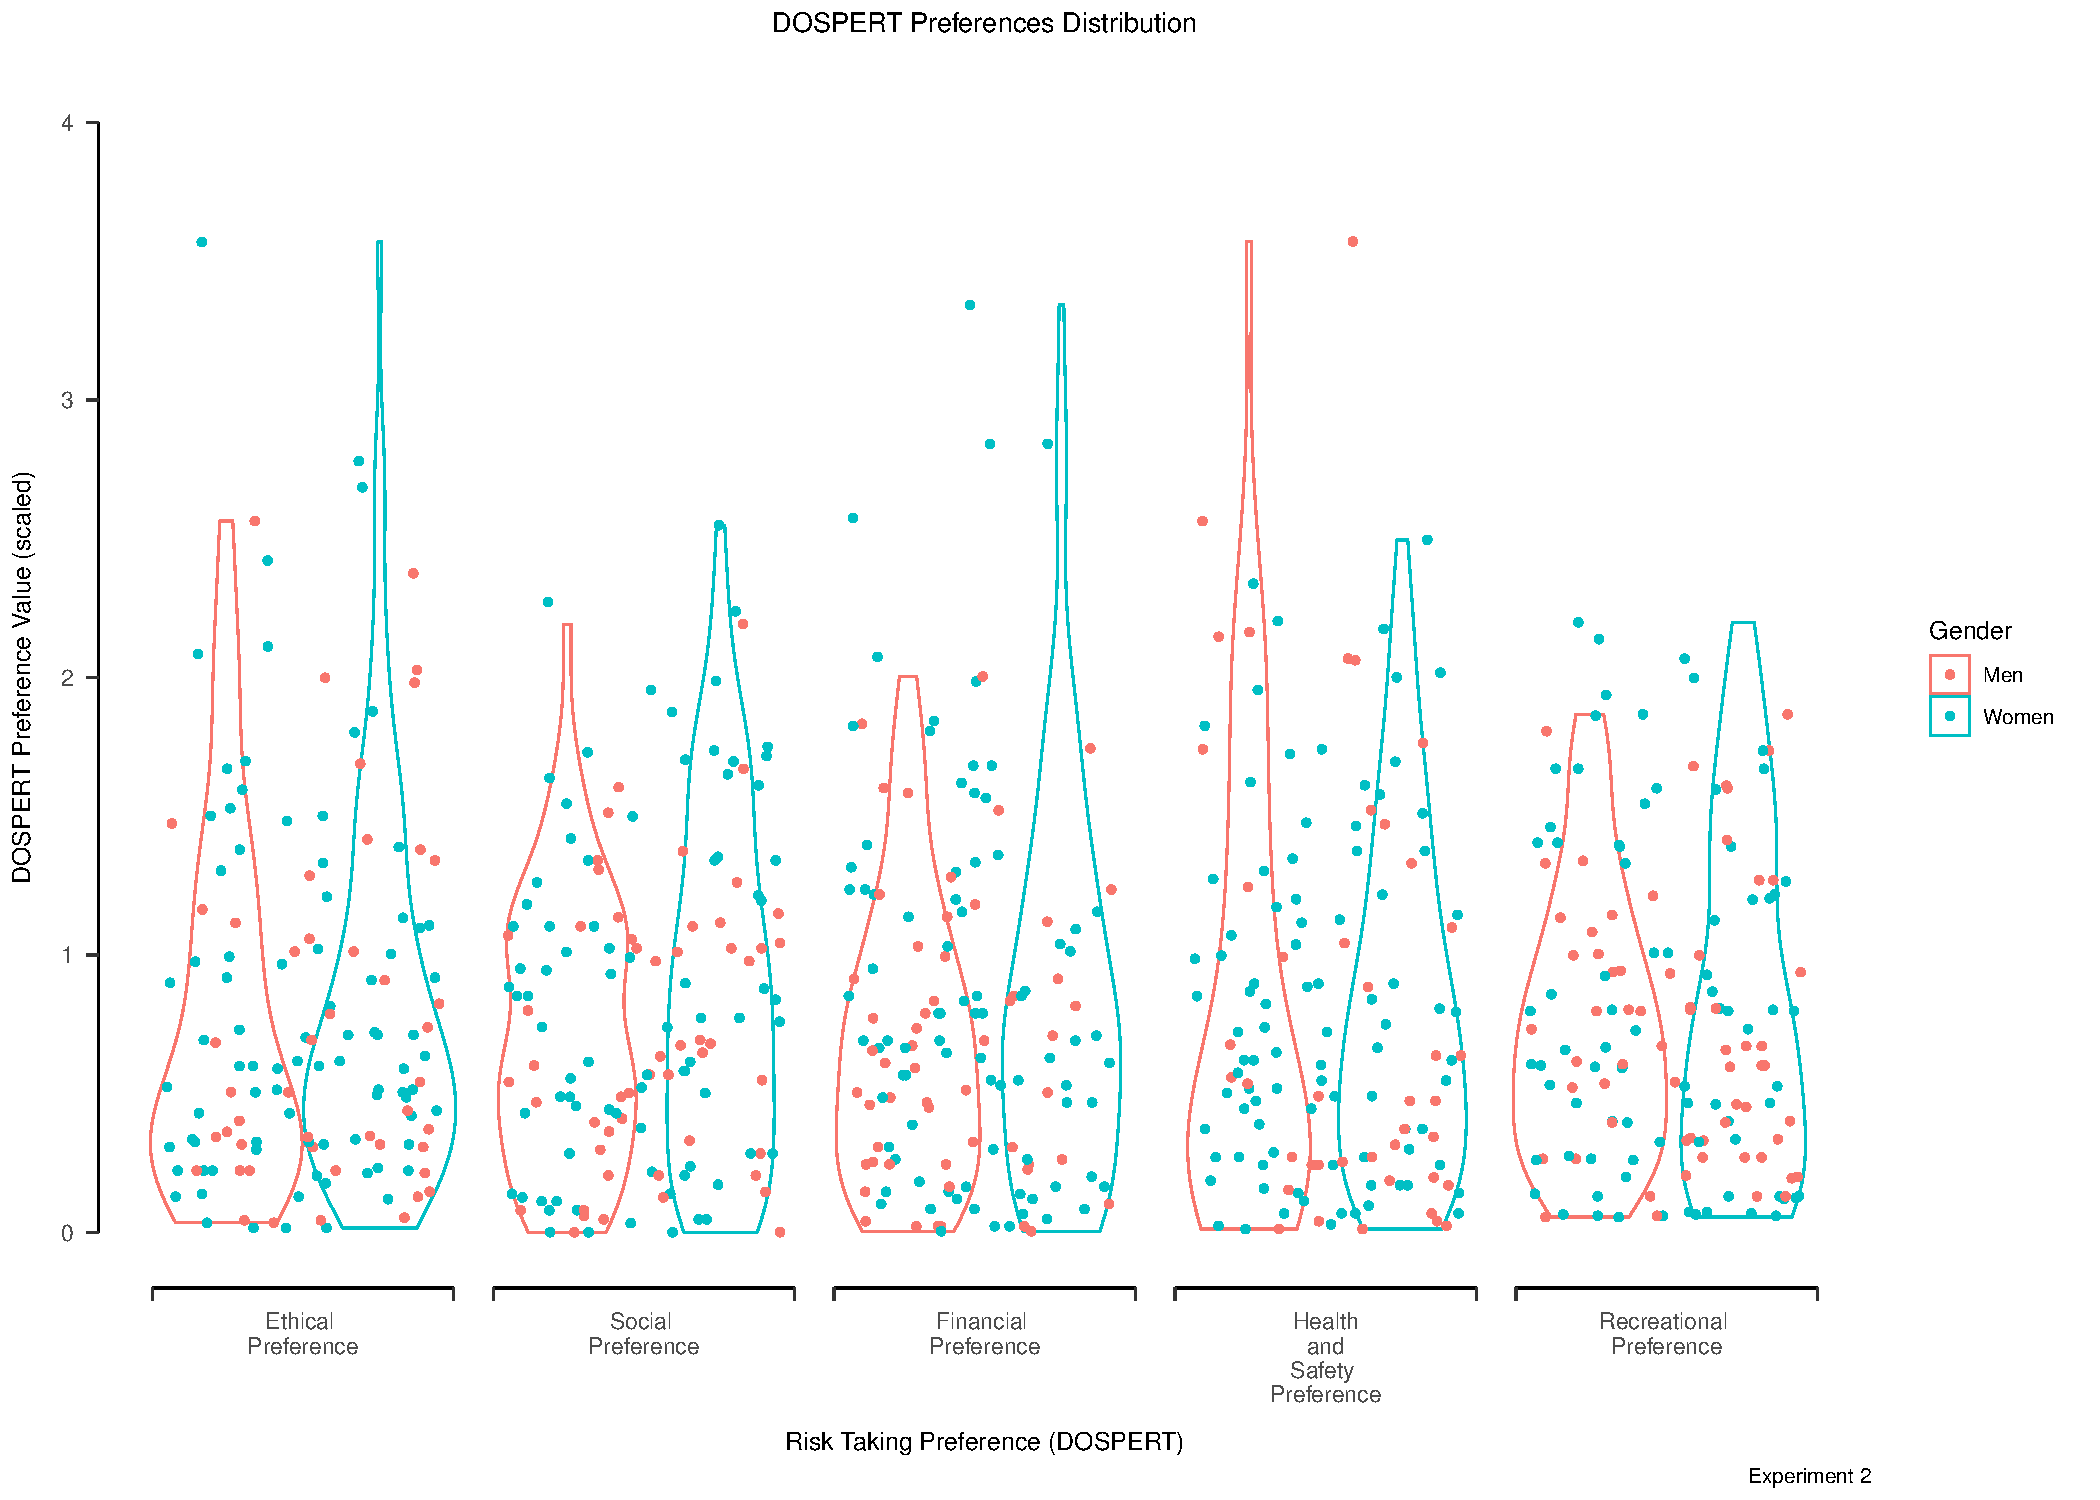
\includegraphics{/Output_Files/Chapter-2-graphs_files/figure-latex/DOSPERT-Preferences-GenderExperiment2-1.pdf}
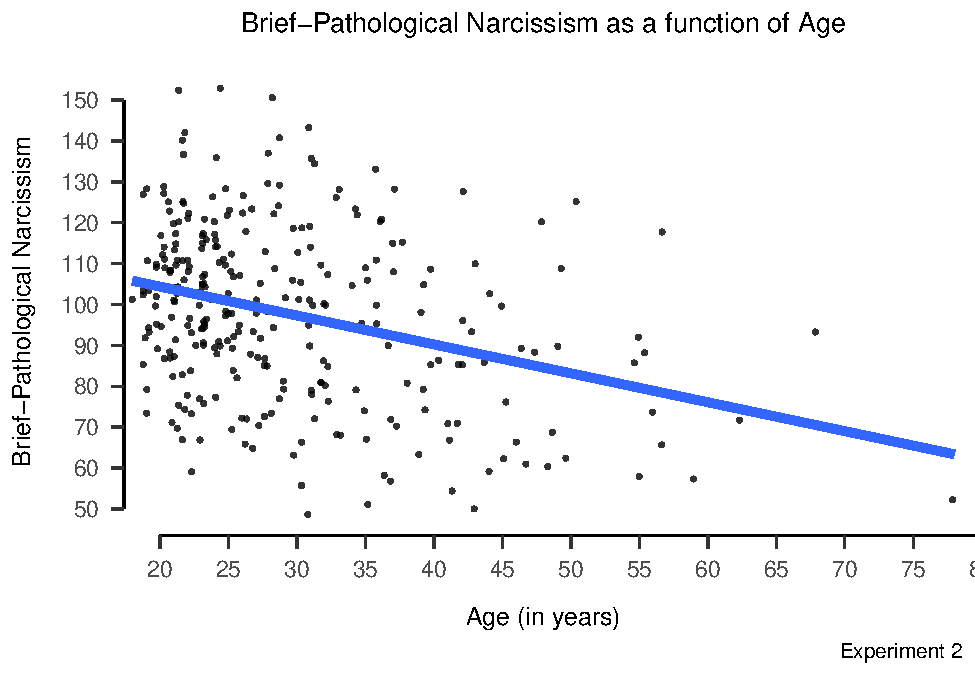
\includegraphics{/Output_Files/Chapter-2-graphs_files/figure-latex/Experiment-2-PNI-distribution-1.pdf}
\newpage

\begin{landscape}
\begin{figure}

{\centering 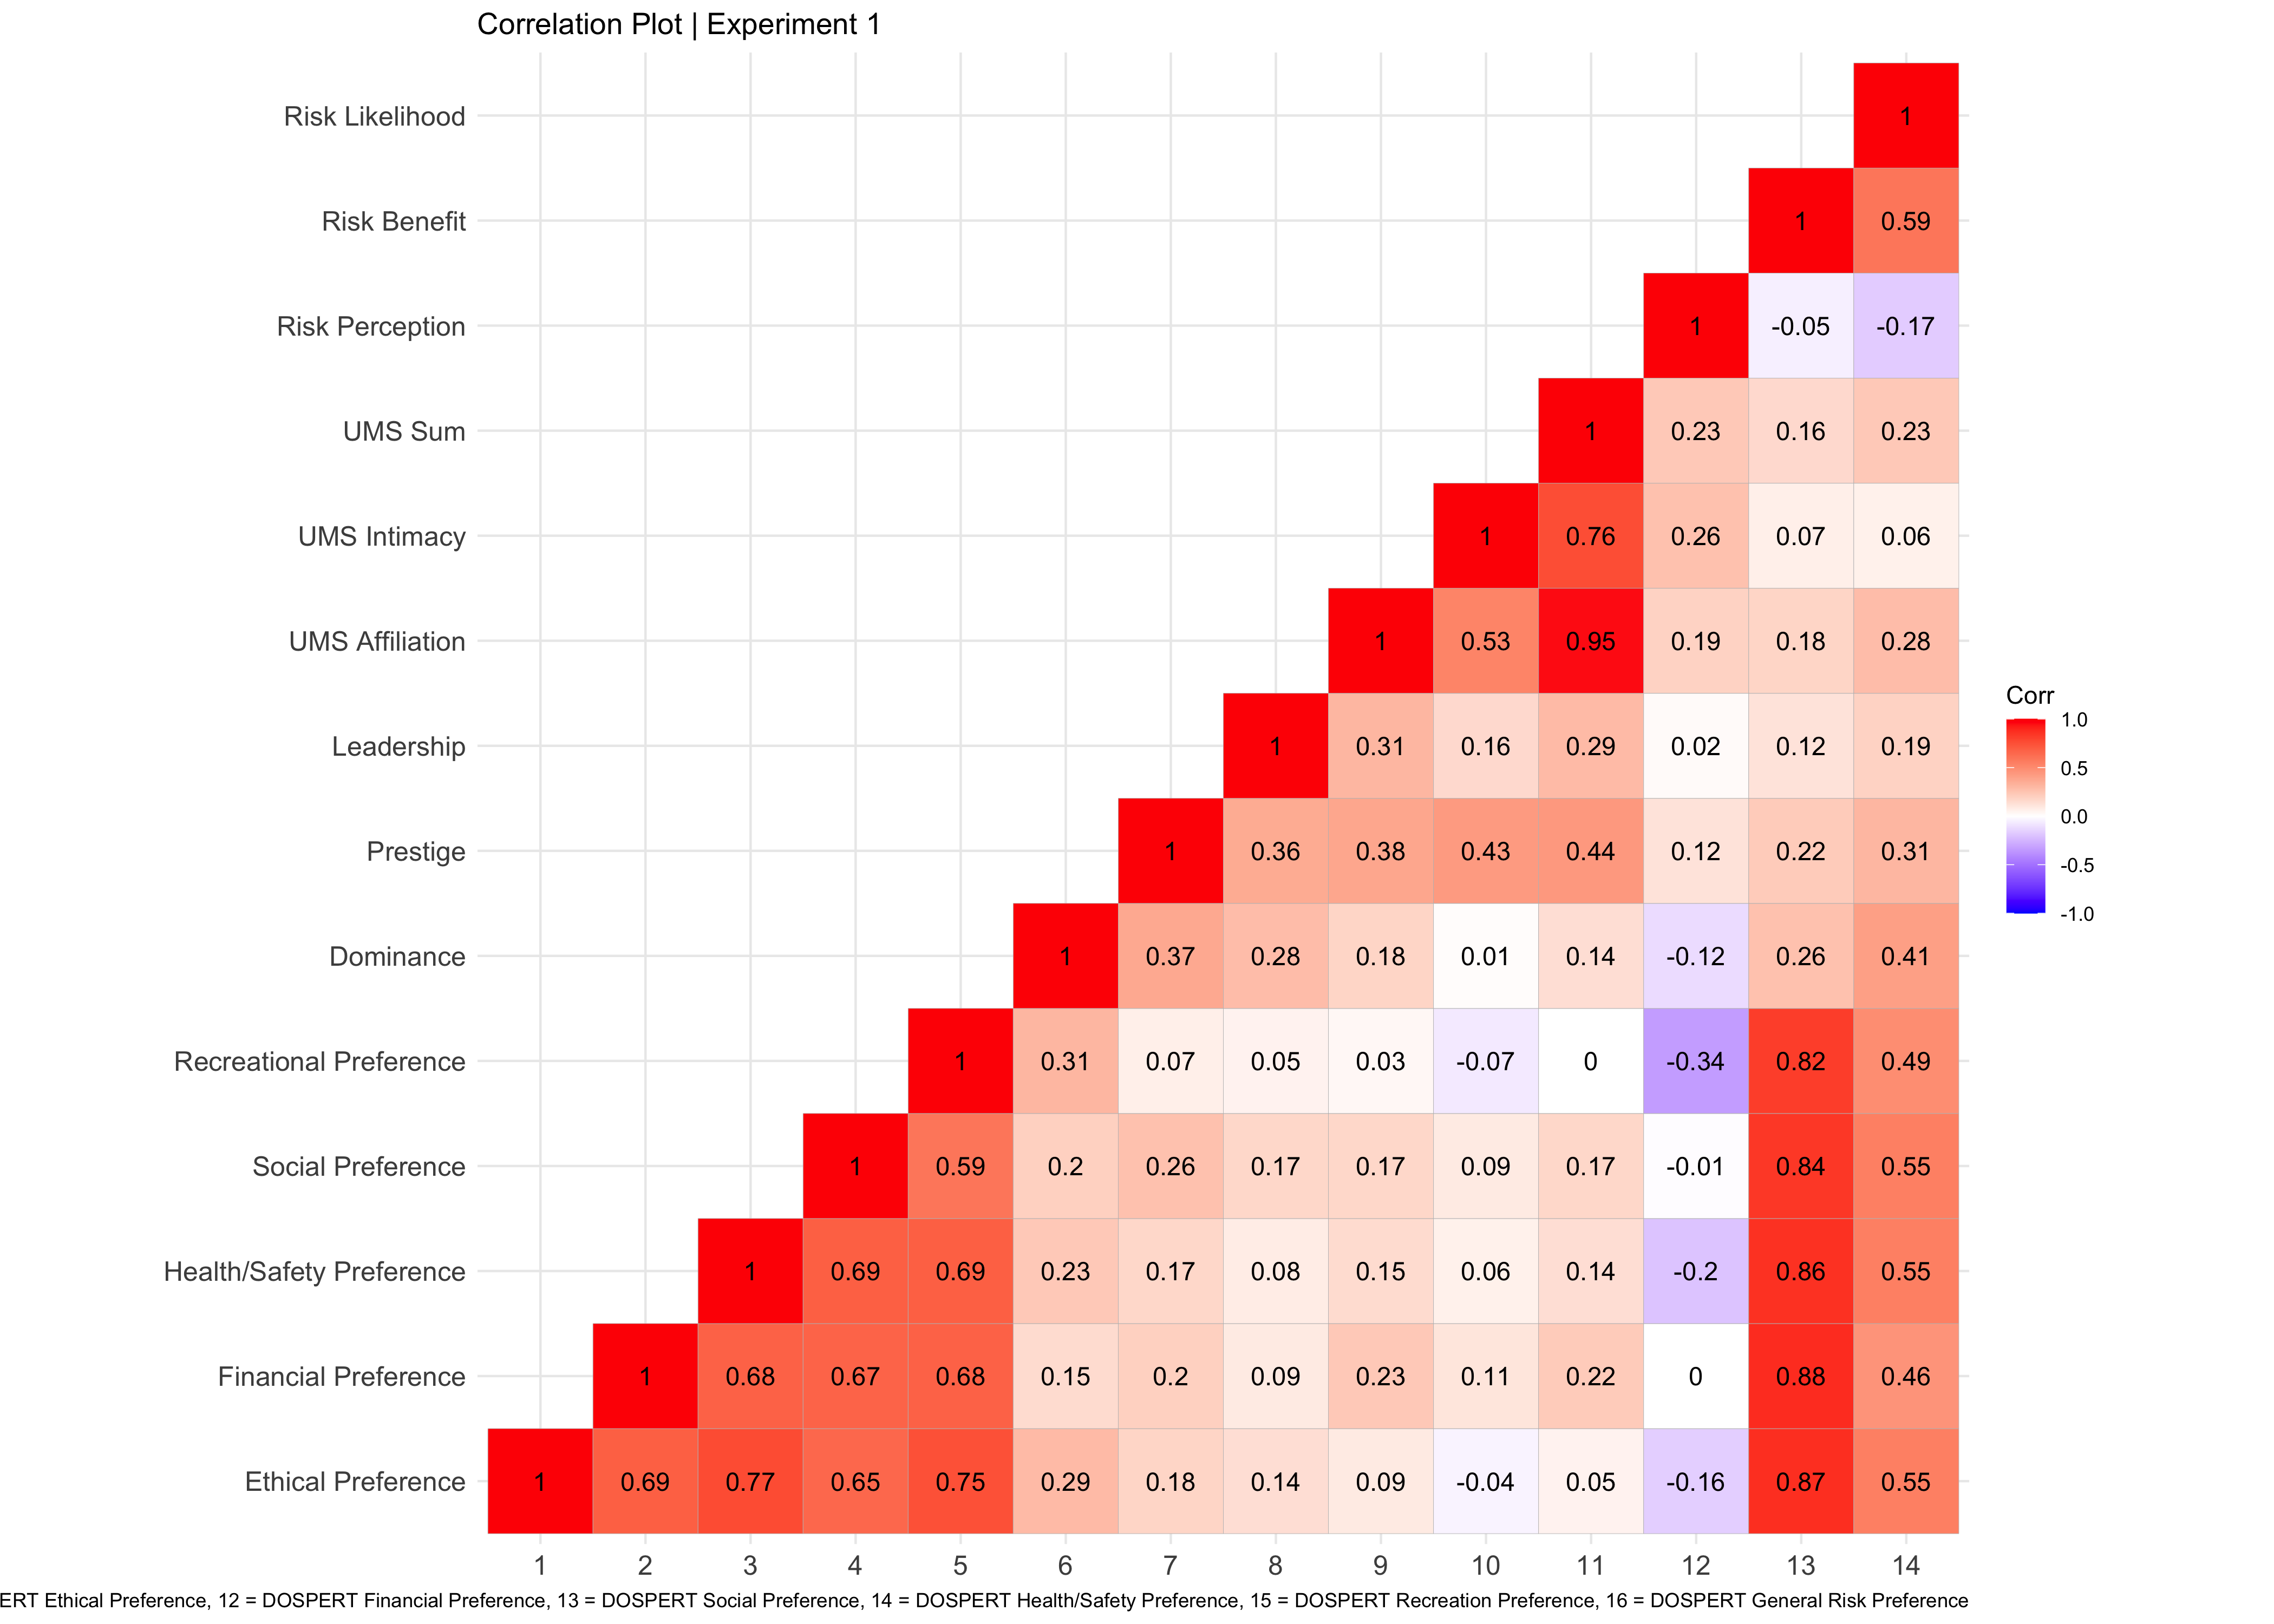
\includegraphics{/Output_Files/Chapter-2-graphs_files/figure-latex/correlationExperiment1-1} 

}

\caption{Depicted here is a correlation plot of the indices of experiment 1. The legend denotes stronger positive correlation (closer to 1 and darker red) or stronger negative correlation (closer to -1 and darker blue).}\label{fig:correlationExperiment1}
\end{figure}
\newpage
\begin{figure}

{\centering 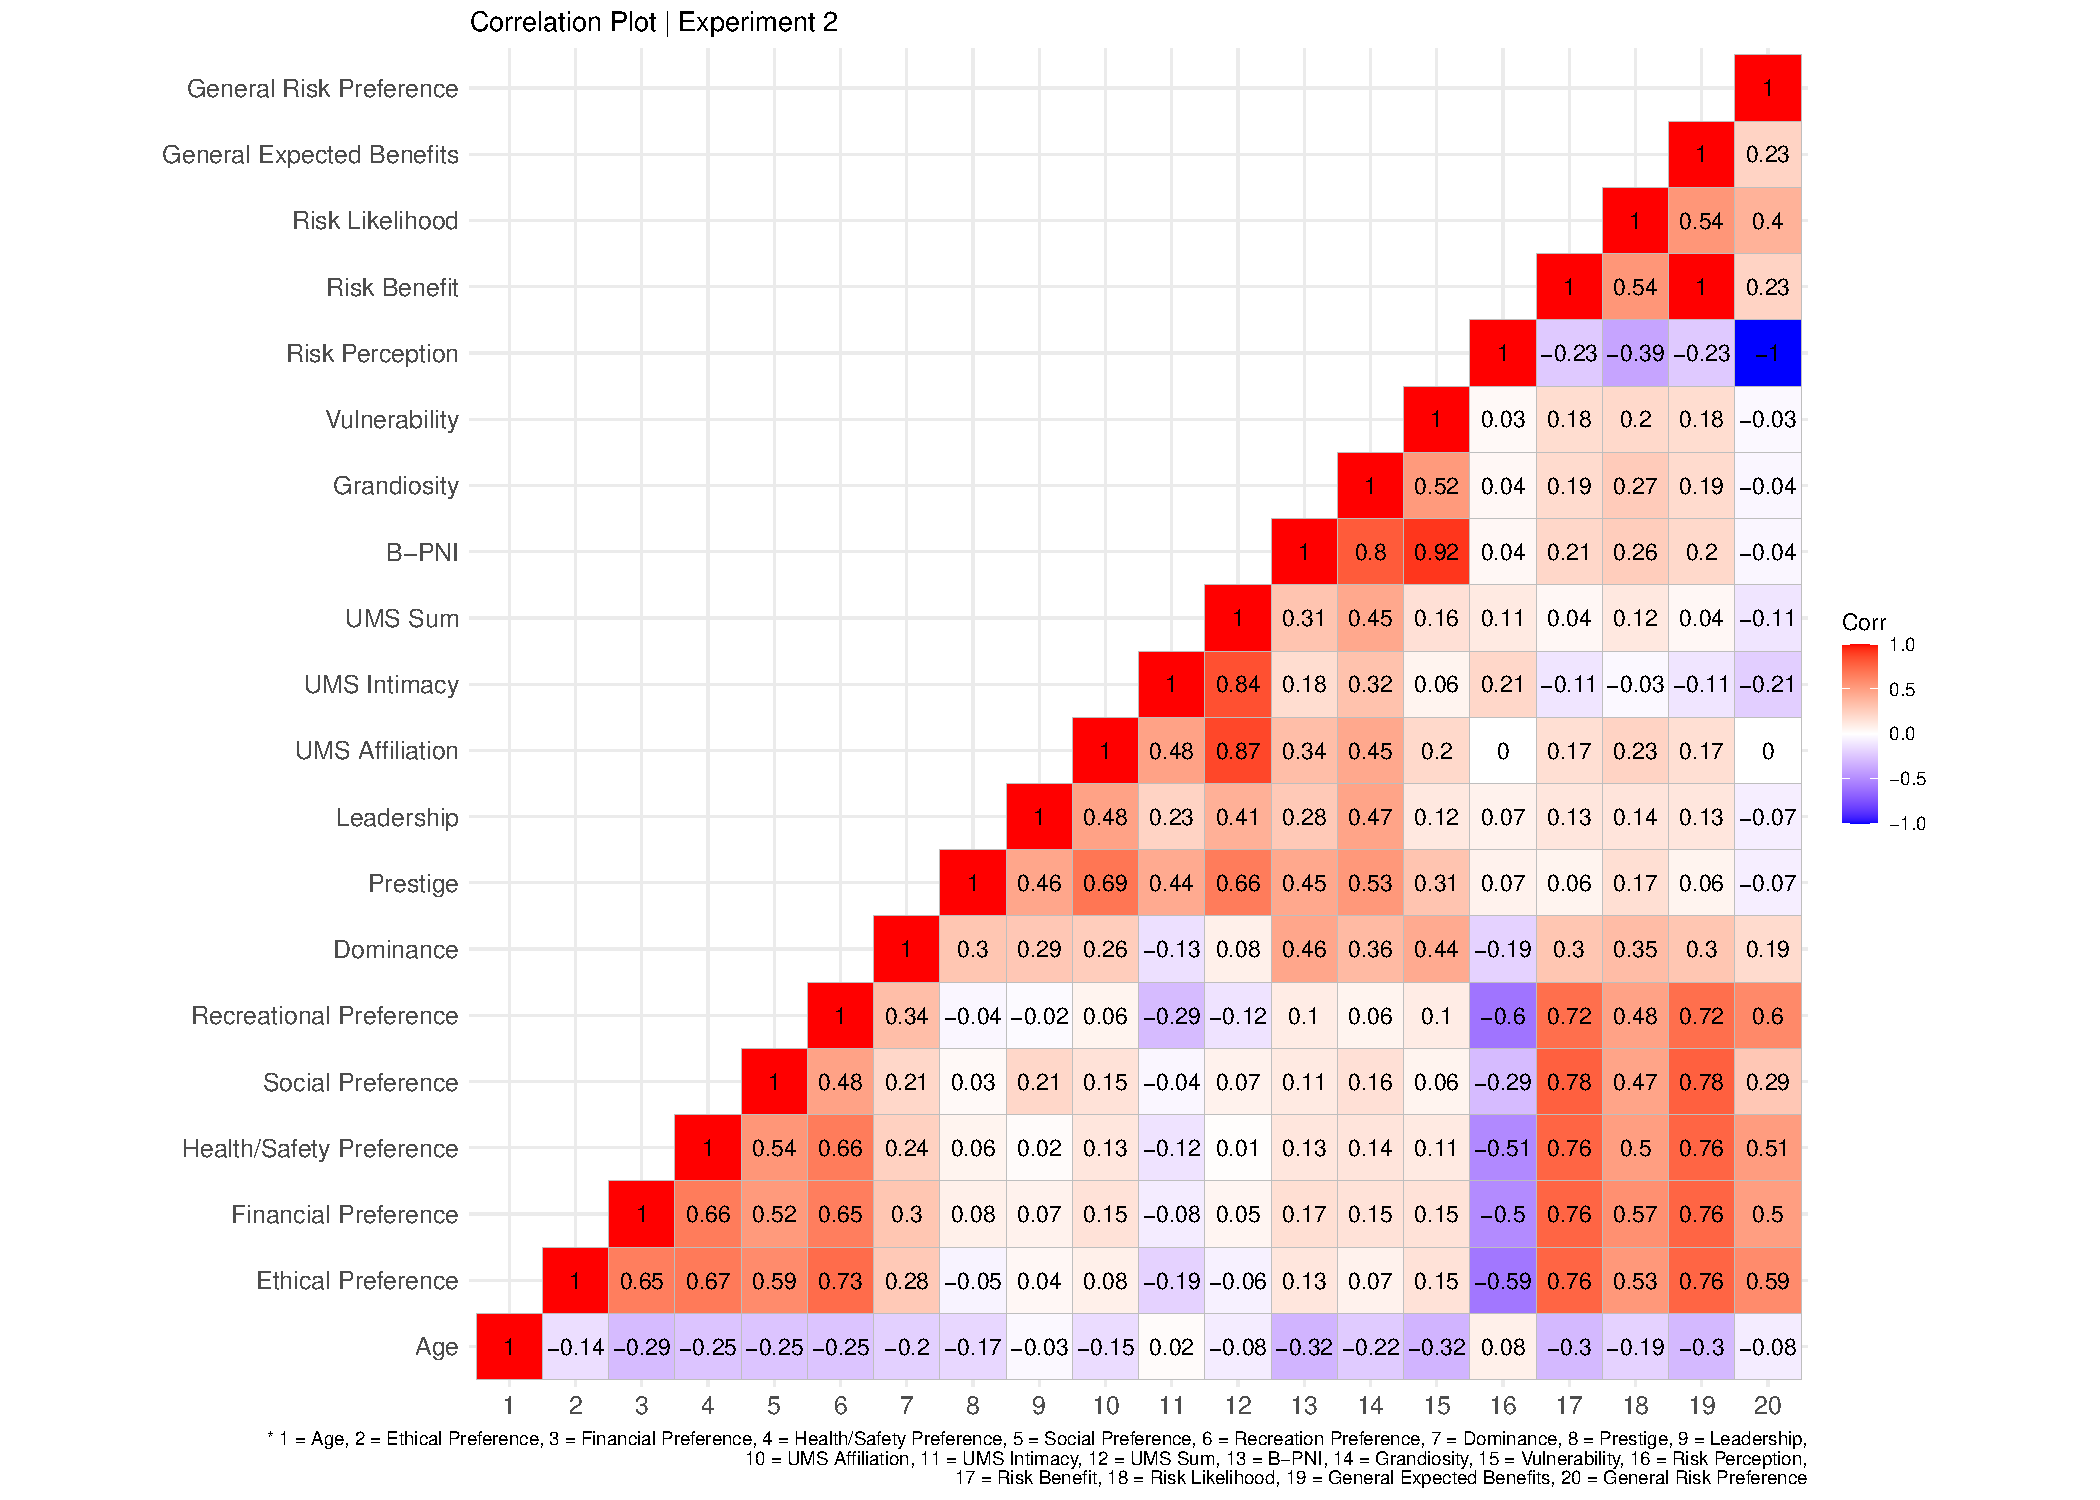
\includegraphics{/Output_Files/Chapter-2-graphs_files/figure-latex/correlationExperiment2-1} 

}

\caption{Depicted here is a correlation plot of the indices of experiment 2. The legend denotes stronger positive correlation (closer to 1 and darker red) or stronger negative correlation (closer to -1 and darker blue).}\label{fig:correlationExperiment2}
\end{figure}
\end{landscape}
\newpage
\begin{figure}

{\centering 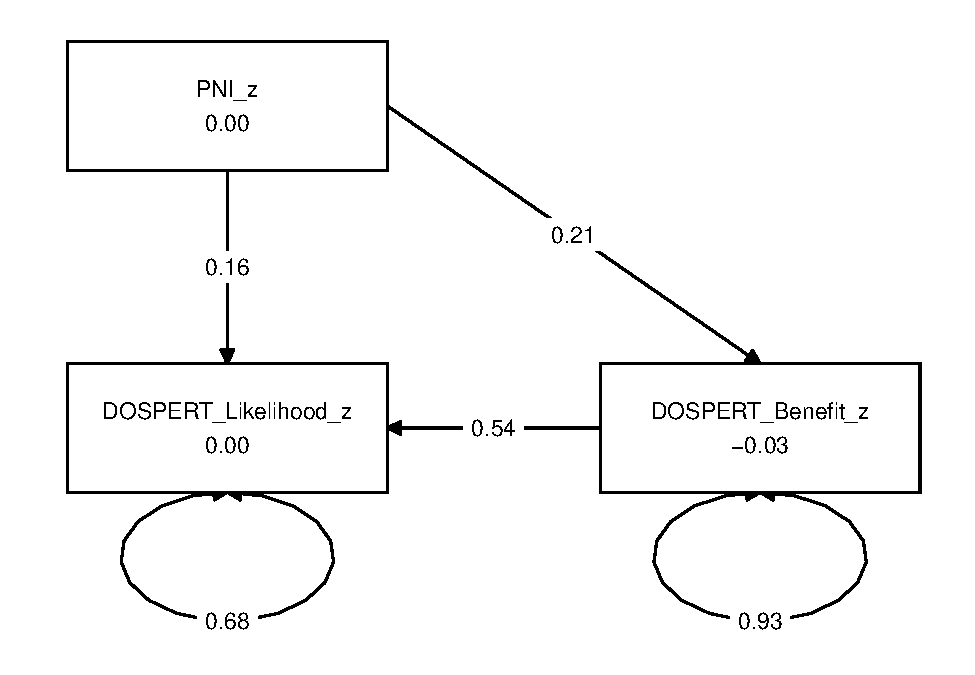
\includegraphics[width=1\linewidth]{/Output_Files/Chapter-2-graphs_files/figure-latex/MediationFit1-1} 

}

\caption{Figure represents a mediation model with Narcissism as the central mediator in the model.The outcome variables being risk likelihood.}\label{fig:MediationFit1}
\end{figure}
\begin{figure}

{\centering 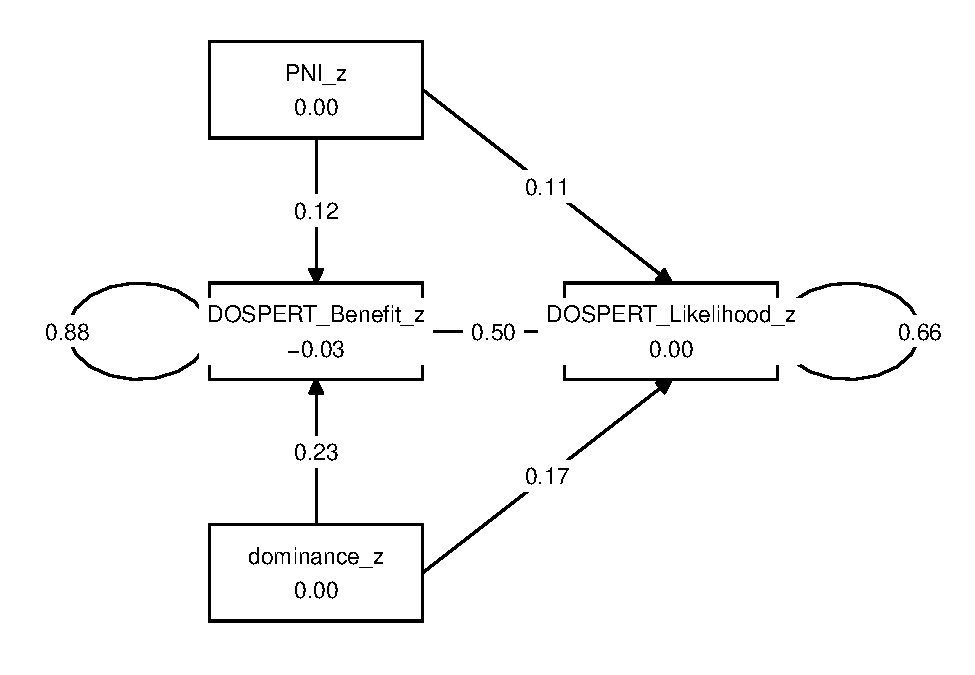
\includegraphics[width=1\linewidth]{/Output_Files/Chapter-2-graphs_files/figure-latex/MediationFit2-1} 

}

\caption{Figure represents a mediation model with Narcissism and Dominance as the central mediators in a parallel model.The outcome variables being risk likelihood.}\label{fig:MediationFit2}
\end{figure}
\begin{figure}

{\centering 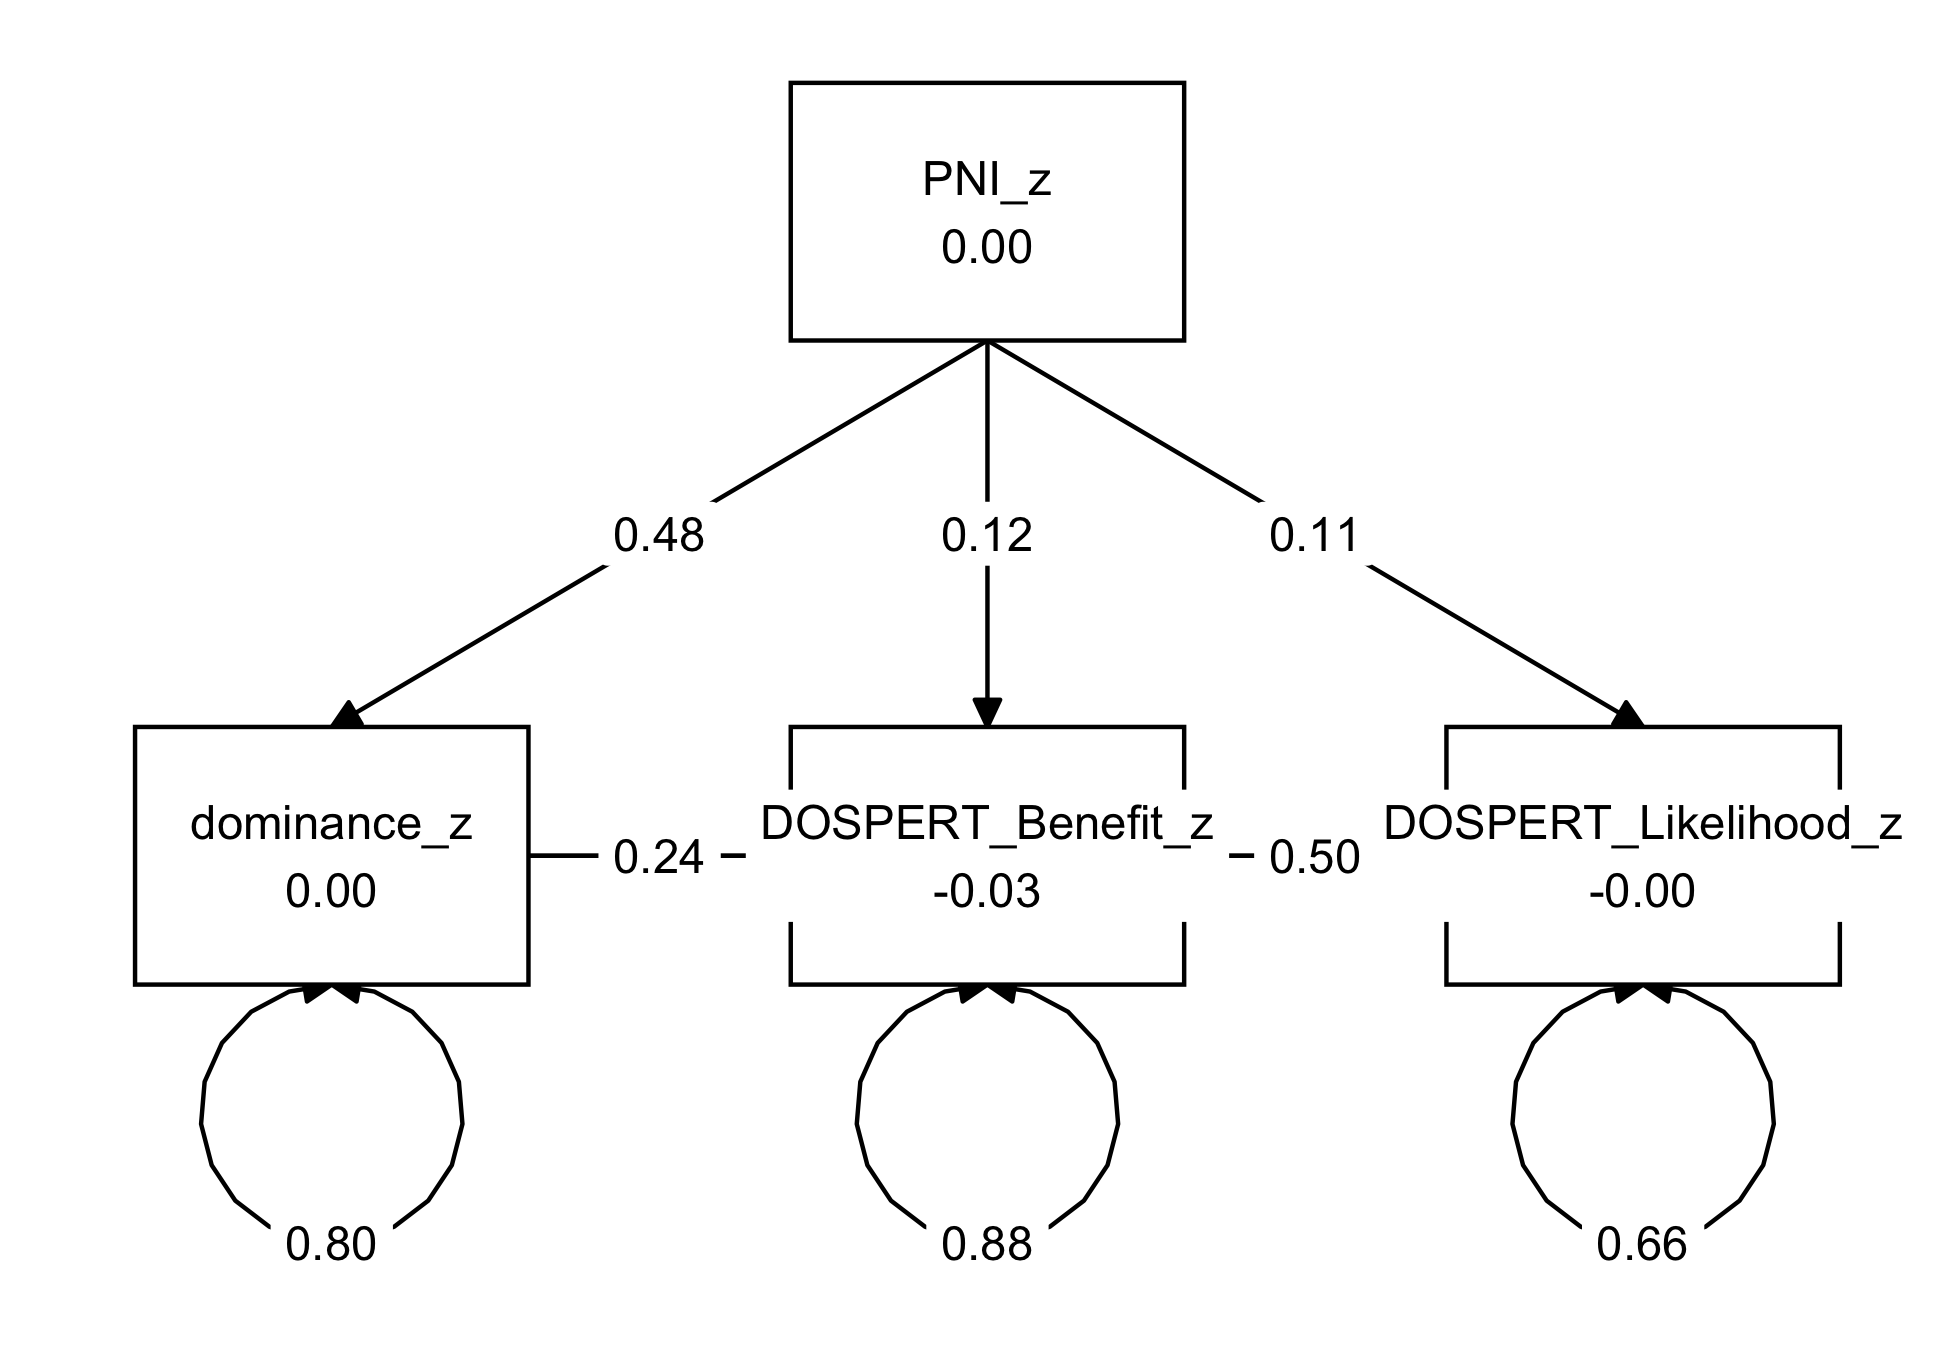
\includegraphics[width=1\linewidth]{/Output_Files/Chapter-2-graphs_files/figure-latex/MediationFit3-1} 

}

\caption{Figure represents a mediation model with Narcissism and Dominance as the moderator in a serial model.The outcome variables being risk likelihood.}\label{fig:MediationFit3}
\end{figure}

\newpage


\clearpage
\renewcommand{\listfigurename}{Figure captions}

\clearpage
\renewcommand{\listtablename}{Table captions}


\end{document}
